\subsection{1.1 SQL语言表达能力的限制}

\begin{frame}[fragile,allowframebreaks]{【任务1】打印课程的所有先修课}
\begin{itemize}
    \item 【任务1】打印“数据库系统概论”课程的所有先修课信息
    \begin{figure}
        \centering
        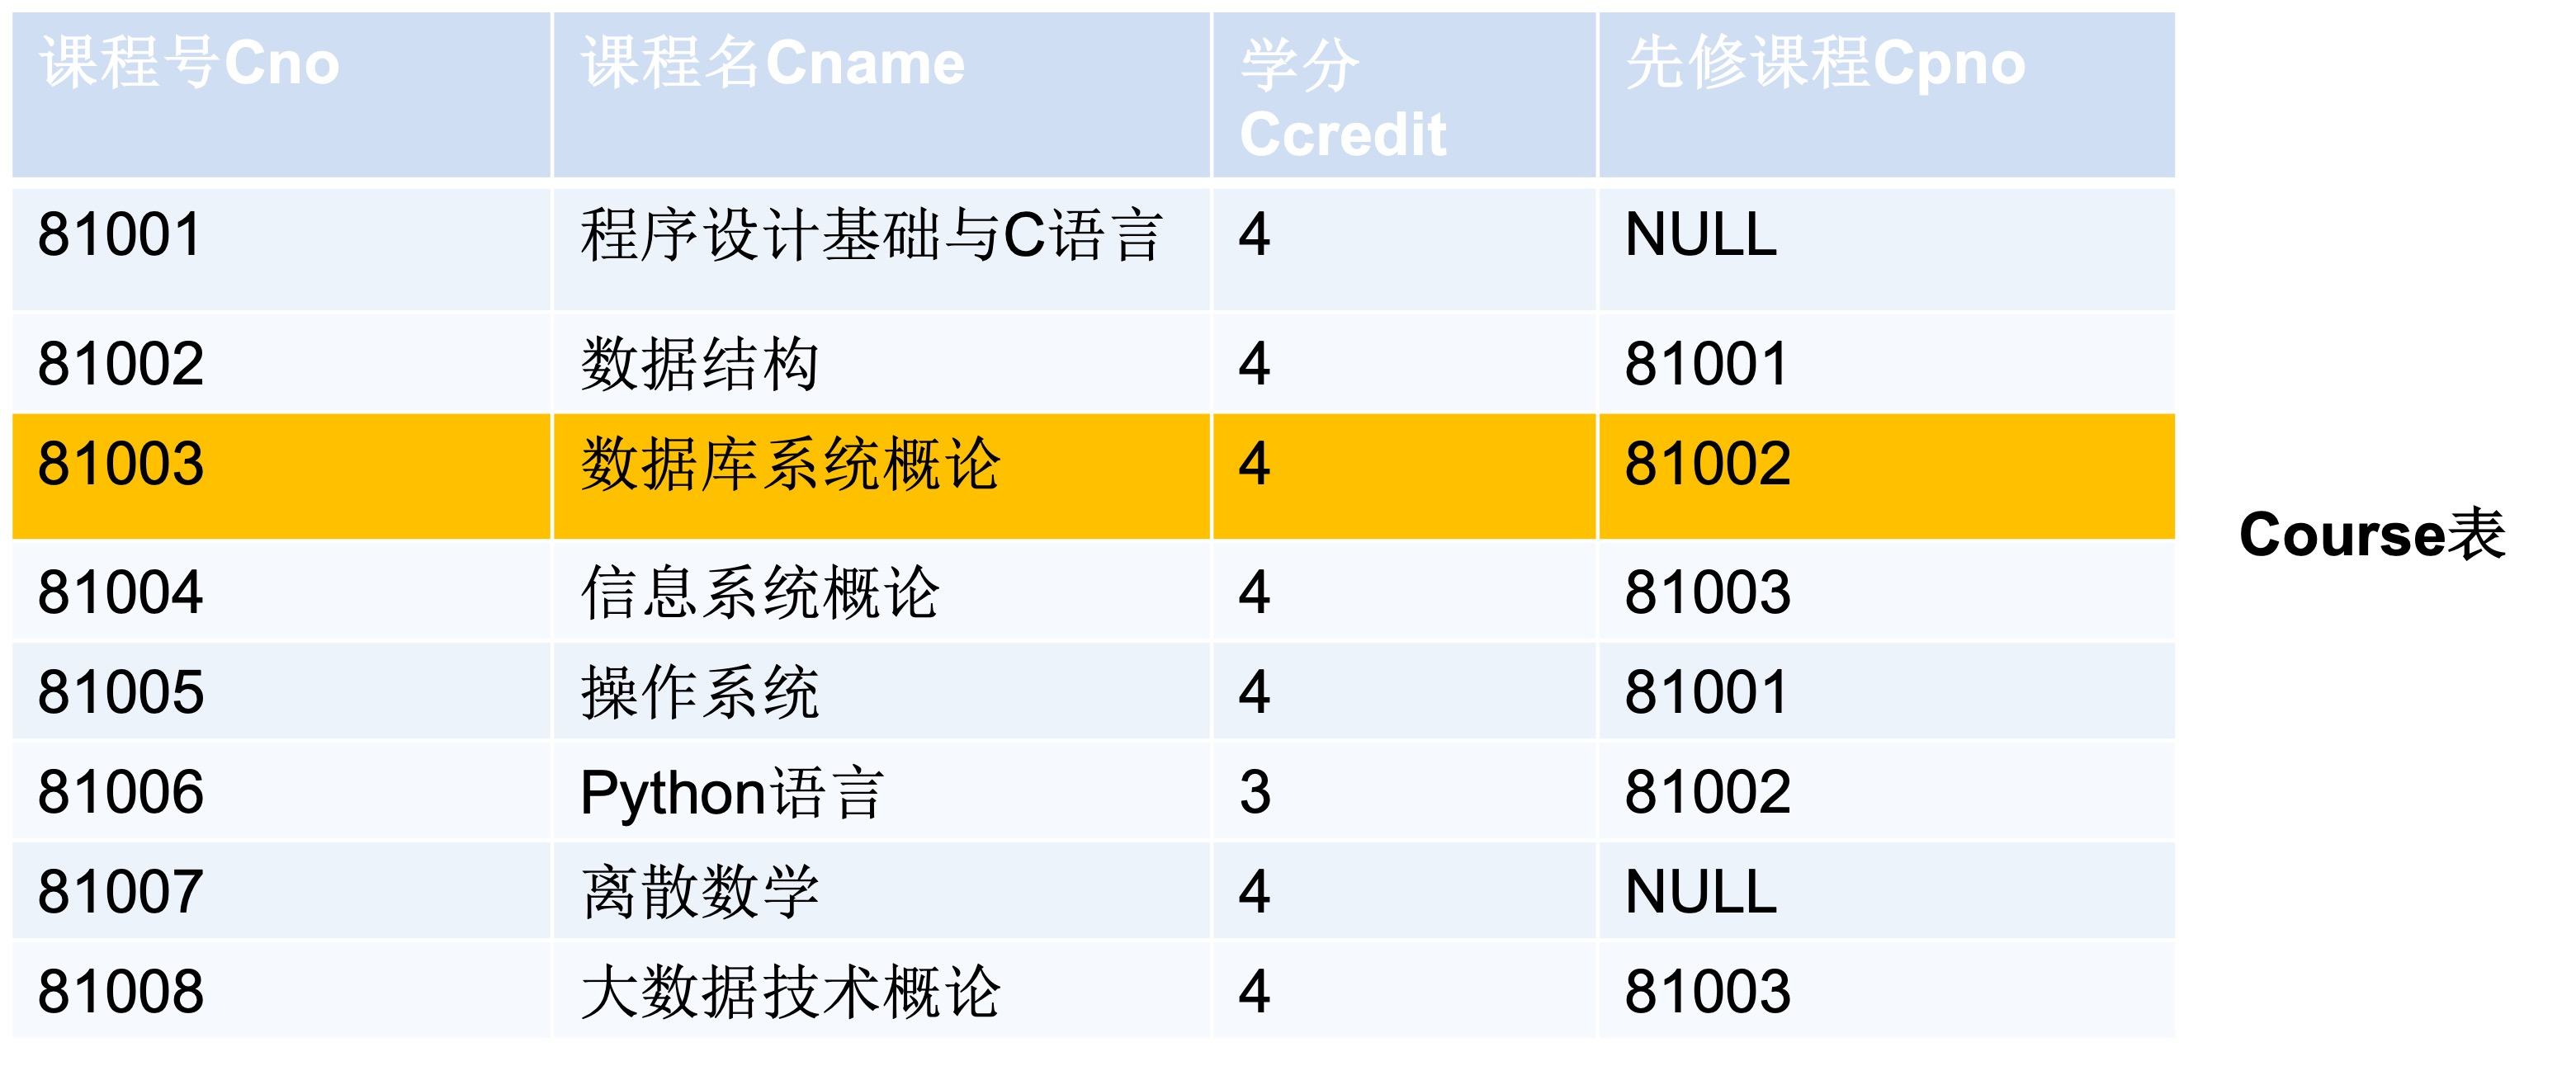
\includegraphics[width=0.8\textwidth]{figure/fig-1.jpg}
    \end{figure}
\framebreak
    
    \item【任务1】打印“数据库系统概论”课程的所有先修课信息

    \begin{figure}
        \centering
        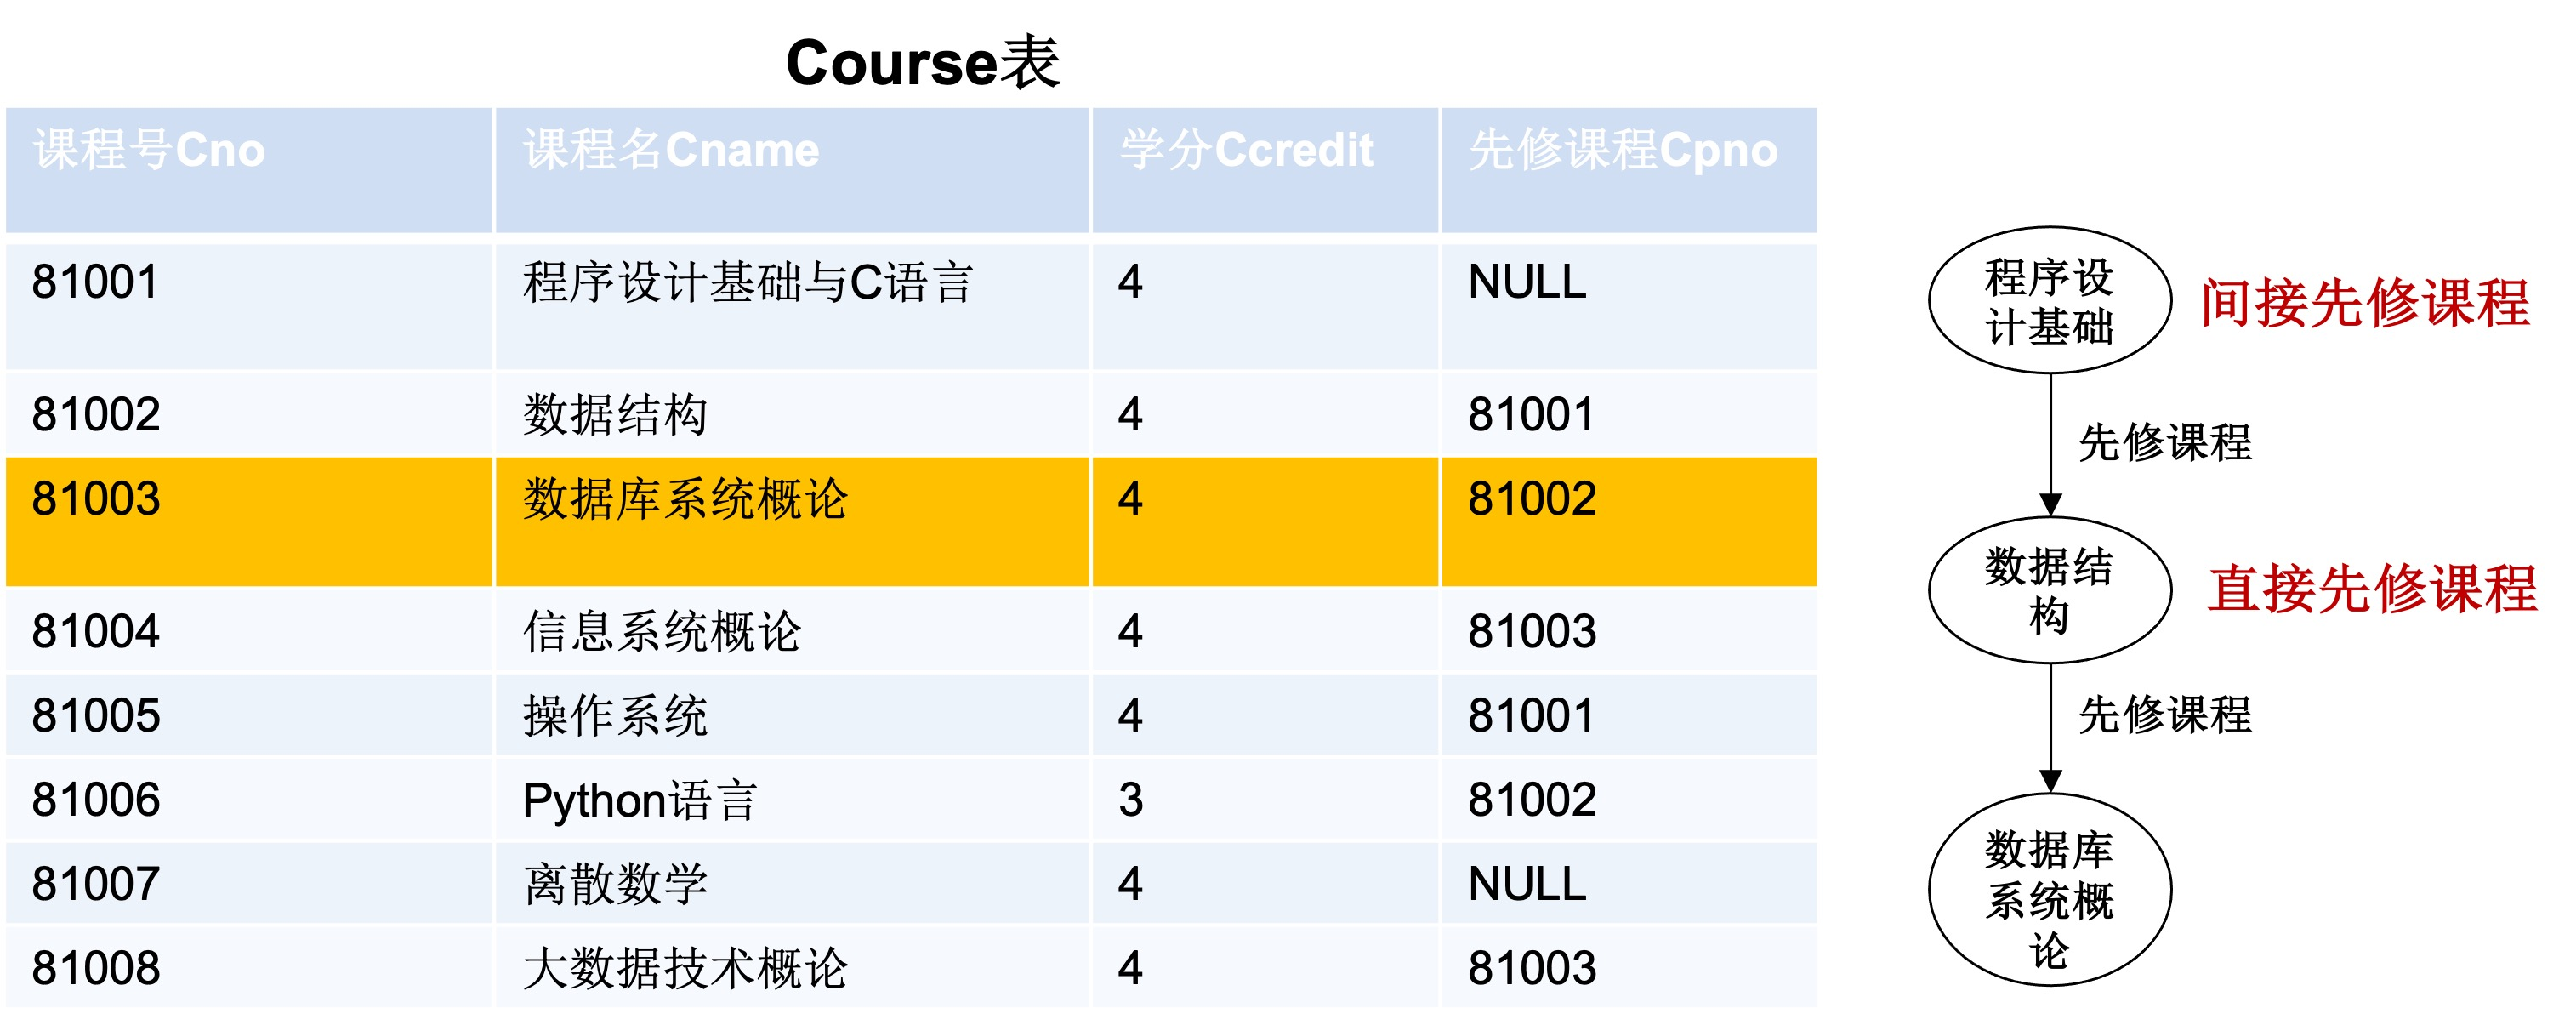
\includegraphics[width=0.8\textwidth]{figure/fig-2.jpg}
    \end{figure}

\framebreak
\item 任务分析:SQL如何表达
    \begin{itemize}
        \item 难点:课程可能同时存在直接先修课和间接先修课
        \item 情况一:如何查询直接先修课:自身连接查询
        \item 情况二:如何查询间接先修课:递归查询\textcolor{red}{(无法表达)}
    \end{itemize}
\end{itemize}
\end{frame}

\begin{frame}[fragile,allowframebreaks]{直接先修课的SQL语句表达}
\begin{itemize}
    \item 如何查询直接先修课:自连接

\begin{enumerate}
    \item 步骤1:找出“数据库系统概论”课程的全部直接先修课:记为L[1];
    如果L[1]为空,则任务一结束
\begin{block}{}
\begin{lstlisting}
SELECT B.Cname 
FROM Course A, Course B
WHERE A.Cname = '数据库系统概论' 
AND A.Cpno=B.Cno;
\end{lstlisting}
\end{block} 
\end{enumerate}
\end{itemize}
\end{frame}

\begin{frame}[fragile,allowframebreaks]{间接先修课的SQL语句表达}
\begin{itemize}
\item 如何查询间接先修课:递归执行

\begin{enumerate}
 \setcounter{enumi}{1}
\item 步骤i (i>=2):找出集合L[i-1]中每一门课程的全部直接先修课,并计算它们的并集,记为L[i]
\item 迭代执行步骤i, 直到并集L[i]为空,输出L[1] $\bigcup \dots \bigcup$ L[i]

\begin{block}{}
\begin{lstlisting}
SELECT B.Cname 
FROM Course A, Course B
WHERE A.Cname = '数据结构' AND A.Cpno=B.Cno;


SELECT B.Cname 
FROM Course A, Course B
WHERE A.Cname = '程序设计基础与C语言' AND A.Cpno=B.Cno;
\end{lstlisting}
\end{block} 

\end{enumerate}


\begin{itemize}
    \item 在第2章图2.1所示的Course 表中,执行步骤1,找出“数据库系统概论”课程的直接先修课“数据结构”,即为L[1]
    \item 执行步骤2,找出“数据结构”课程的先修课“程序设计基础与C语言”,即为L[2]
    \item 步骤3,找出“程序设计基础与C语言”的先修课,得到 L[3]
    \item 可以发现L[3]为空,递归查询结束。根据计算结果L[1]$\bigcup$L[2],任务1的输出如表所示

   \begin{figure}
        \centering
        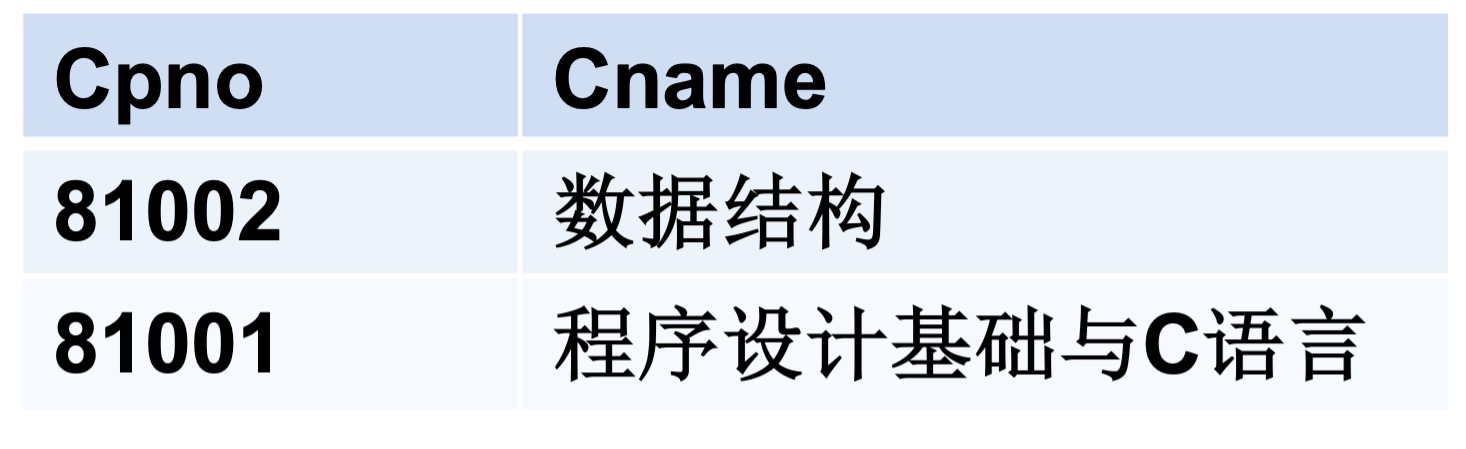
\includegraphics[width=0.5\textwidth]{figure/fig-3.jpg}
    \end{figure}

\end{itemize}

\end{itemize}
\end{frame}




\begin{frame}[allowframebreaks]{【任务2】打印一周内将过生日的学生信息}
\begin{itemize}
    \item 【任务2】打印一周内将过生日的学生信息
   \begin{figure}
        \centering
        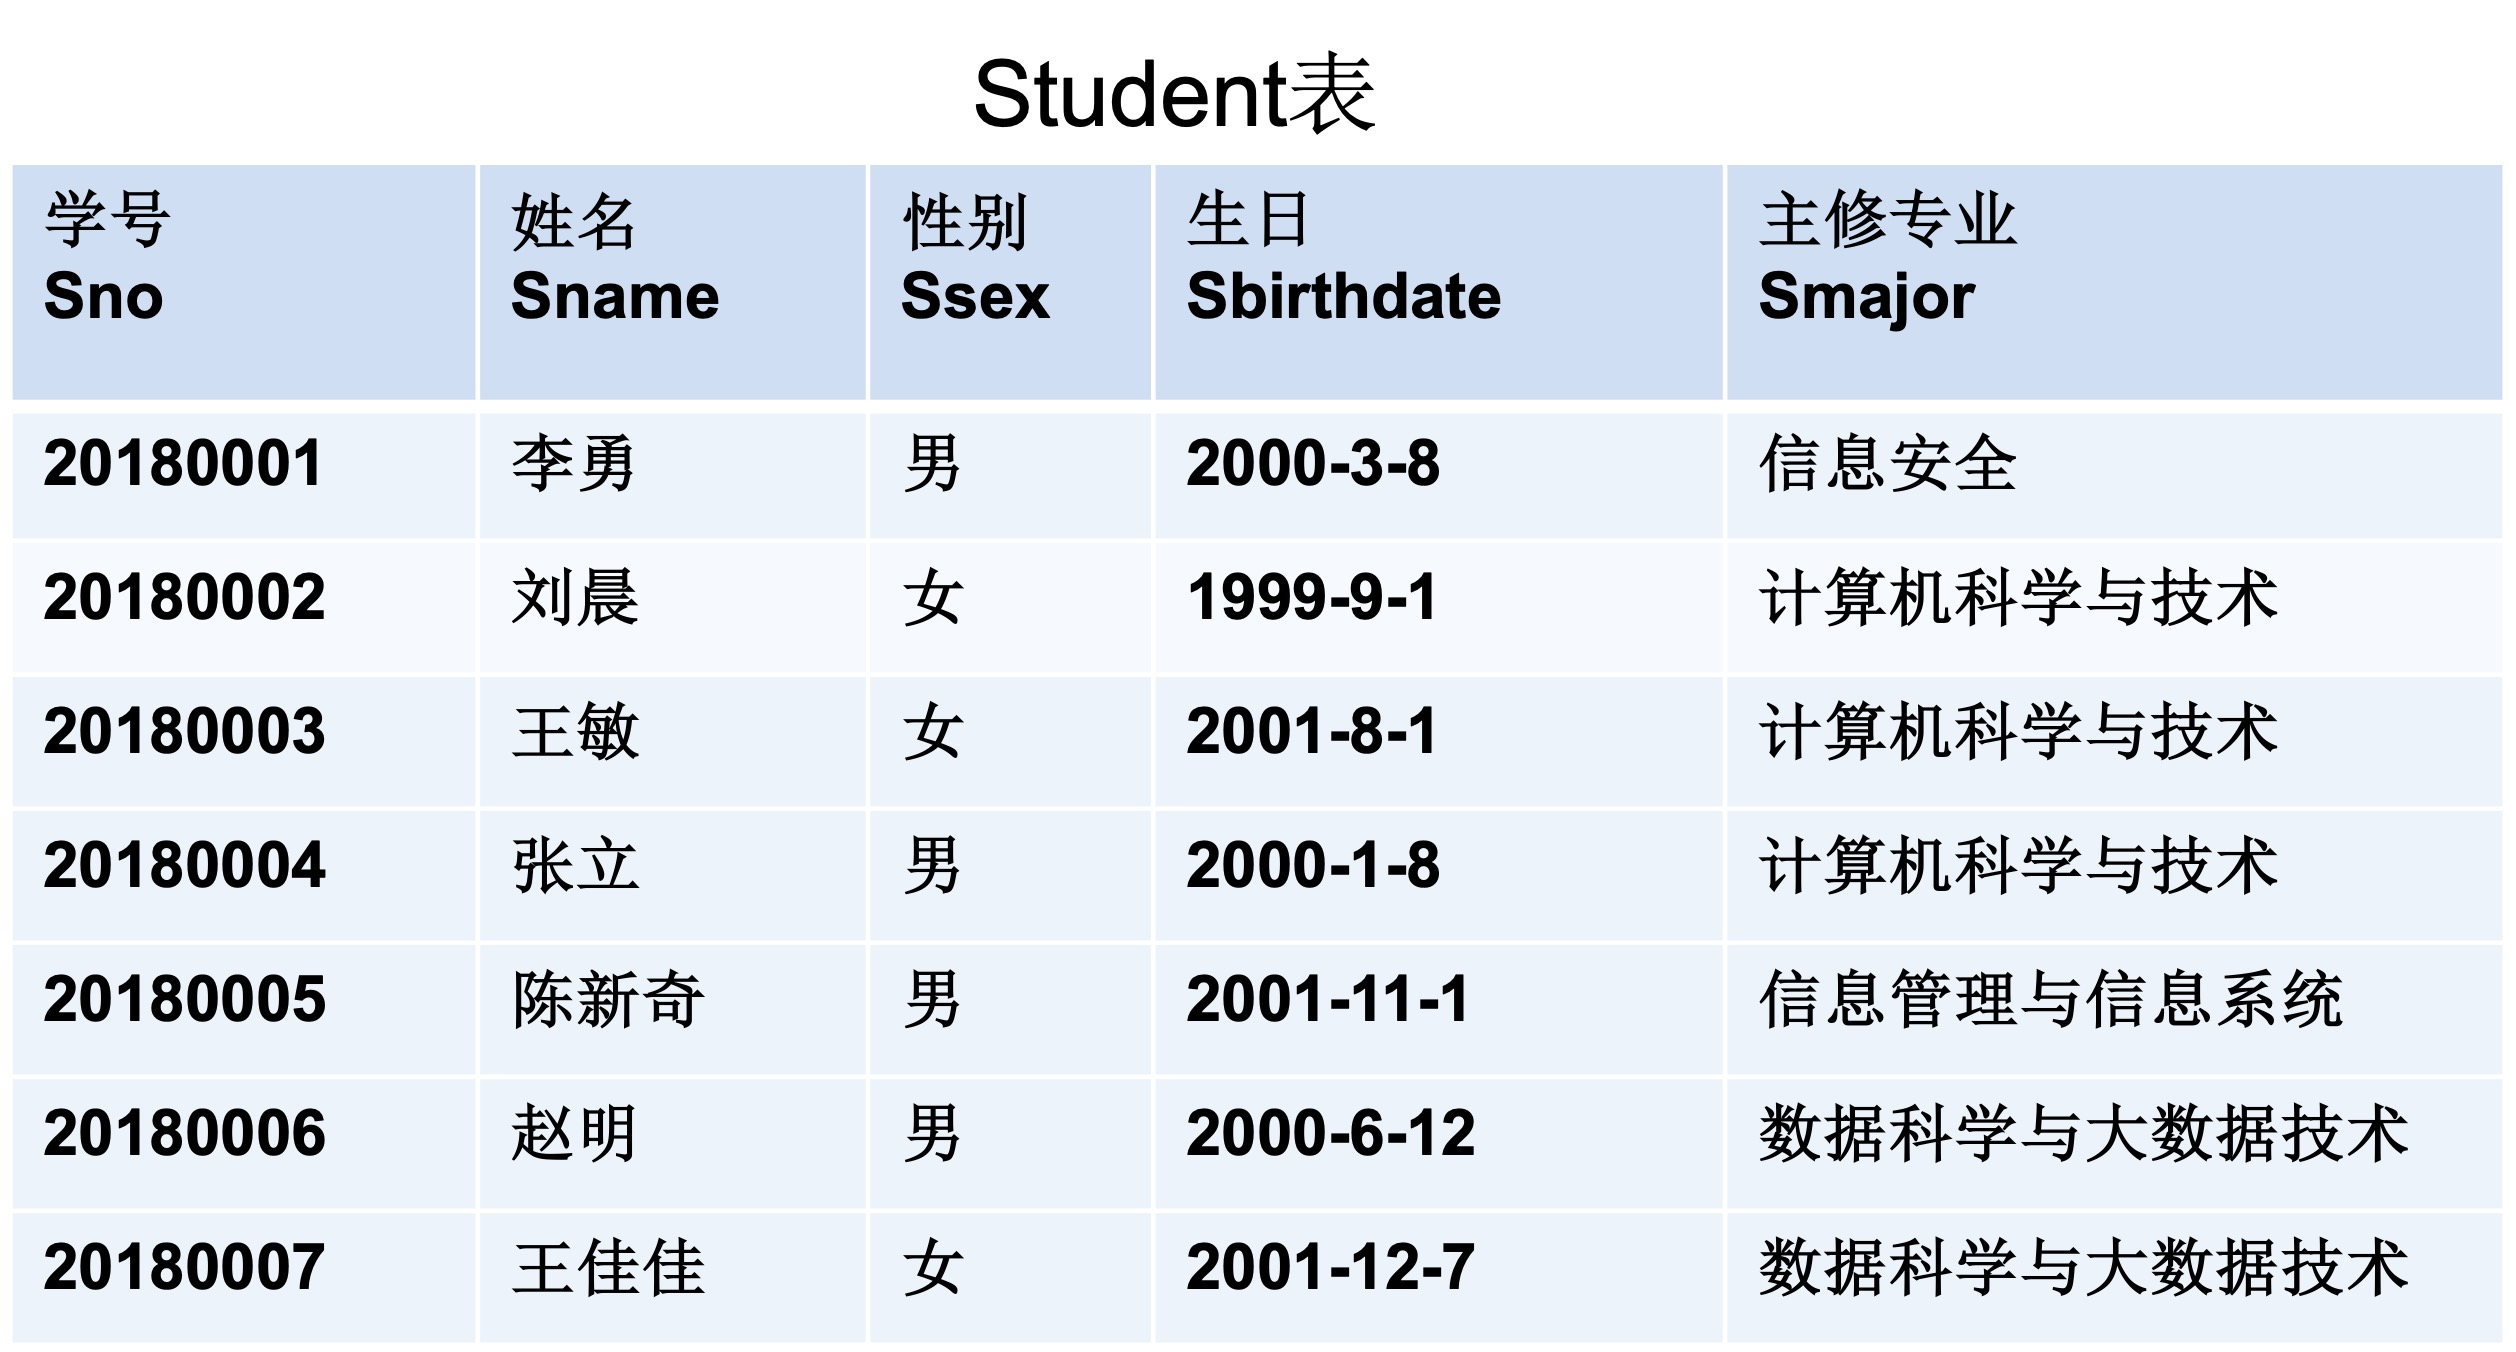
\includegraphics[width=0.7\textwidth]{figure/fig-4.jpg}
    \end{figure}
\end{itemize}

\framebreak
\begin{itemize}
    \item 任务分析:SQL如何表达
\begin{itemize}
    \item 任务2需要数据库系统提供内置函数(本任务主要是日期数)。其求解思路为:扫指个学生的出生日期,例如 2000-6-12,并执行以下步骤
    \begin{enumerate}
\item 把出生日期的年份换成当前日期所在的年份(例如2021),即2021-6-12
\item 获取当前系统的日期,例如 2021-6-9
\item 确定过生日的日期范围[2021-6-9,2021-6-16],即以当前日期为下界,当	前日期后的第七天作为上界
\item 判断出生日期是否在上述日期范围内,如果是,输出该学生信息
    \end{enumerate}
\end{itemize}
\end{itemize}
    
\end{frame}

\begin{frame}[allowframebreaks]{【任务3】计算学生的平均学分绩点GPA}
\begin{itemize}
    \item 【任务3】给定学生学号,计算学生的平均学分绩点GPA
\begin{figure}
    \centering
    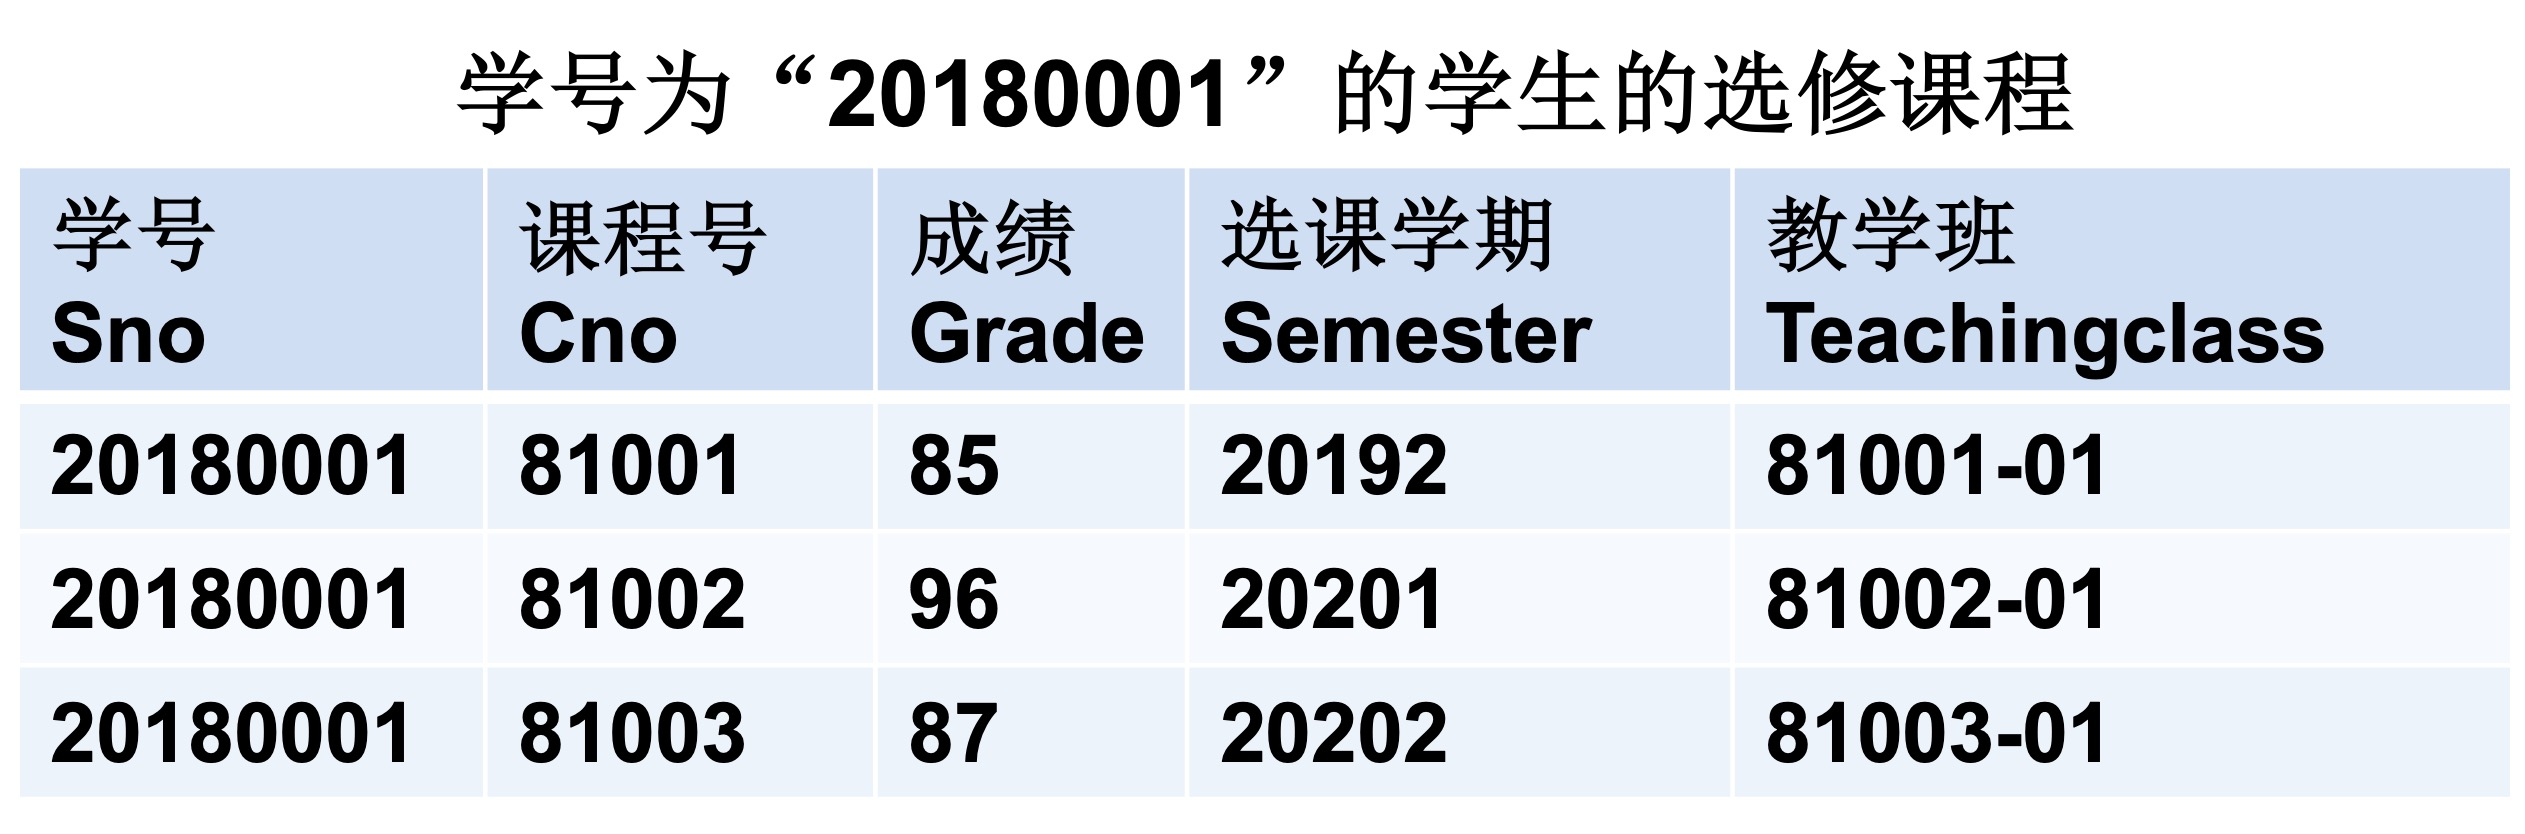
\includegraphics[width=0.8\textwidth]{figure/fig-5.jpg}
\end{figure}

\framebreak
\item 任务分析:SQL如何表达
    \begin{itemize}
    \item 难点:需要用户自主设计业务处理逻辑?
    \item 本任务的求解思路:给定学生学号,找出该学生所有选修课程的学分、成绩;
    \item 根据每门课程的成绩,参照“成绩和绩点对照表”,确定该成绩所处的范围,找出该门课程对应的绩点。
    \end{itemize}
\end{itemize}

\end{frame}

\begin{frame}[allowframebreaks]{【任务4】教学评价浏览与反馈}
\begin{itemize}
    \item 【任务4】教学评价浏览与反馈:学生通过交互界面提交对某一位任课老师的教学评价意见,教师浏览这些评价意见并提供反馈信息
\begin{figure}
    \centering
    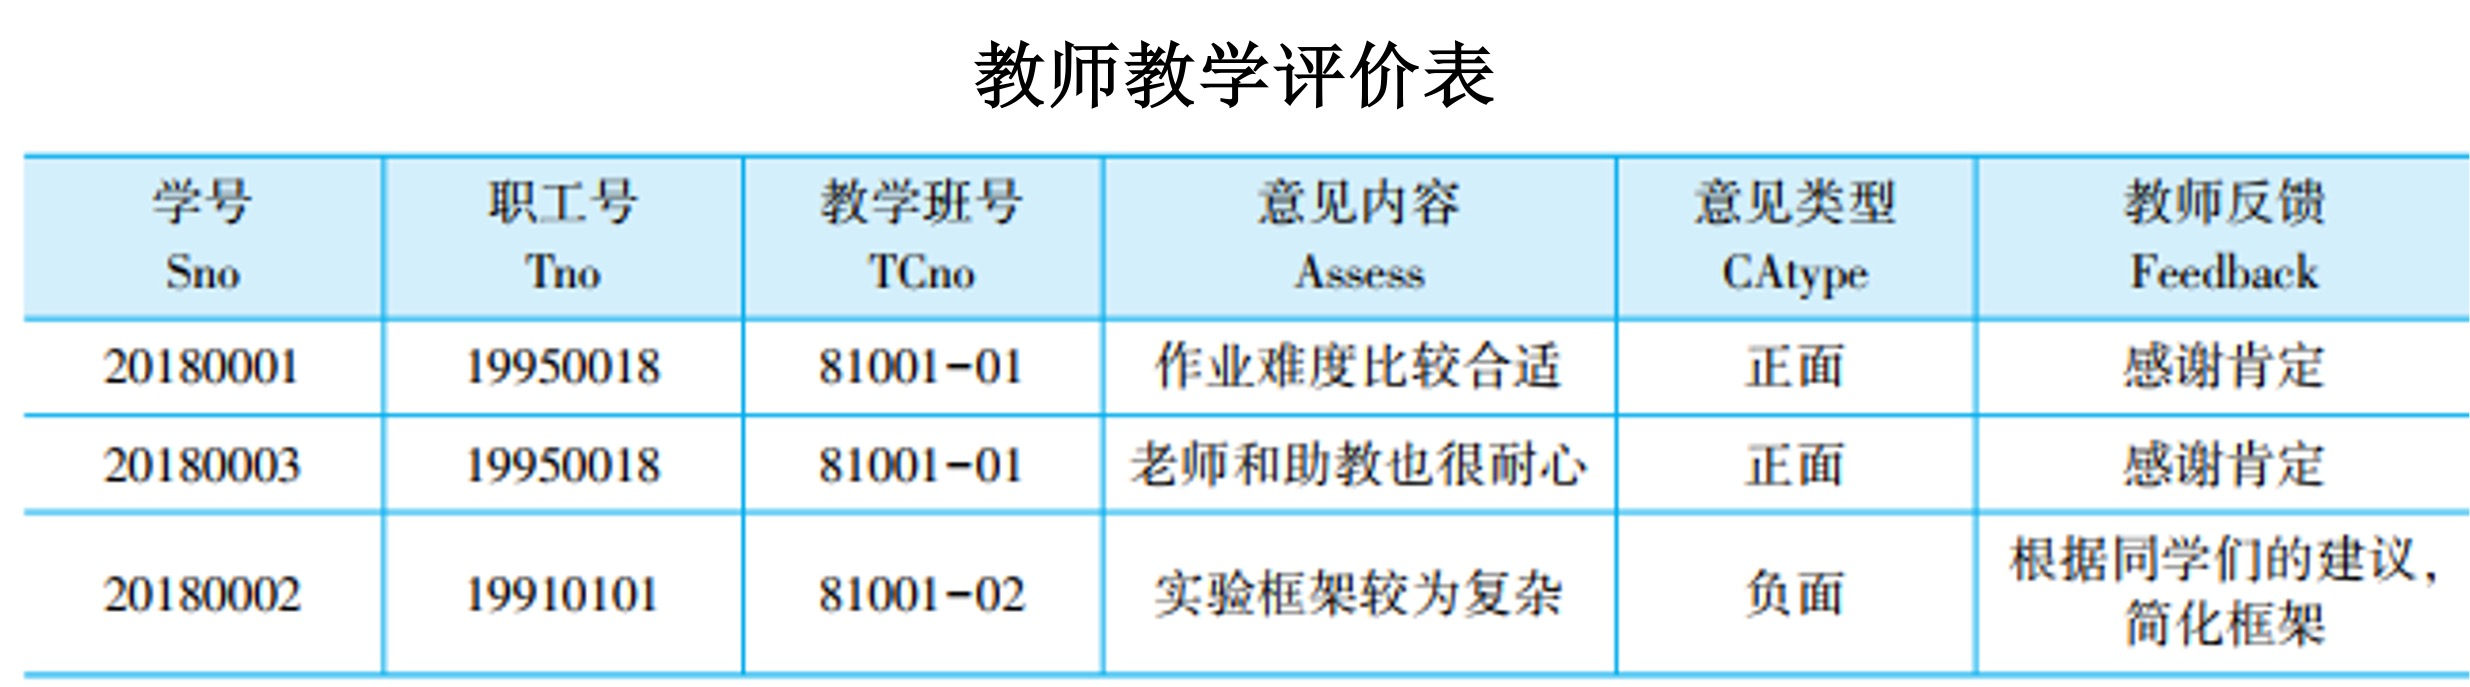
\includegraphics[width=0.8\textwidth]{figure/fig-6.jpg}
\end{figure}
\framebreak
    \item 任务分析:SQL如何表达
\begin{itemize}
    \item 难点:需要建立交互功能
    \item 一方面,学生需要找到指定的教学班和授课教师,建立如图所示的交互界面并输入课程评价。
    \item 另一方面,还要建立如图所示的交互界面,教师浏览教学班学生的评价意见,并针对每条评价逐一做出回复
\begin{figure}
    \centering
    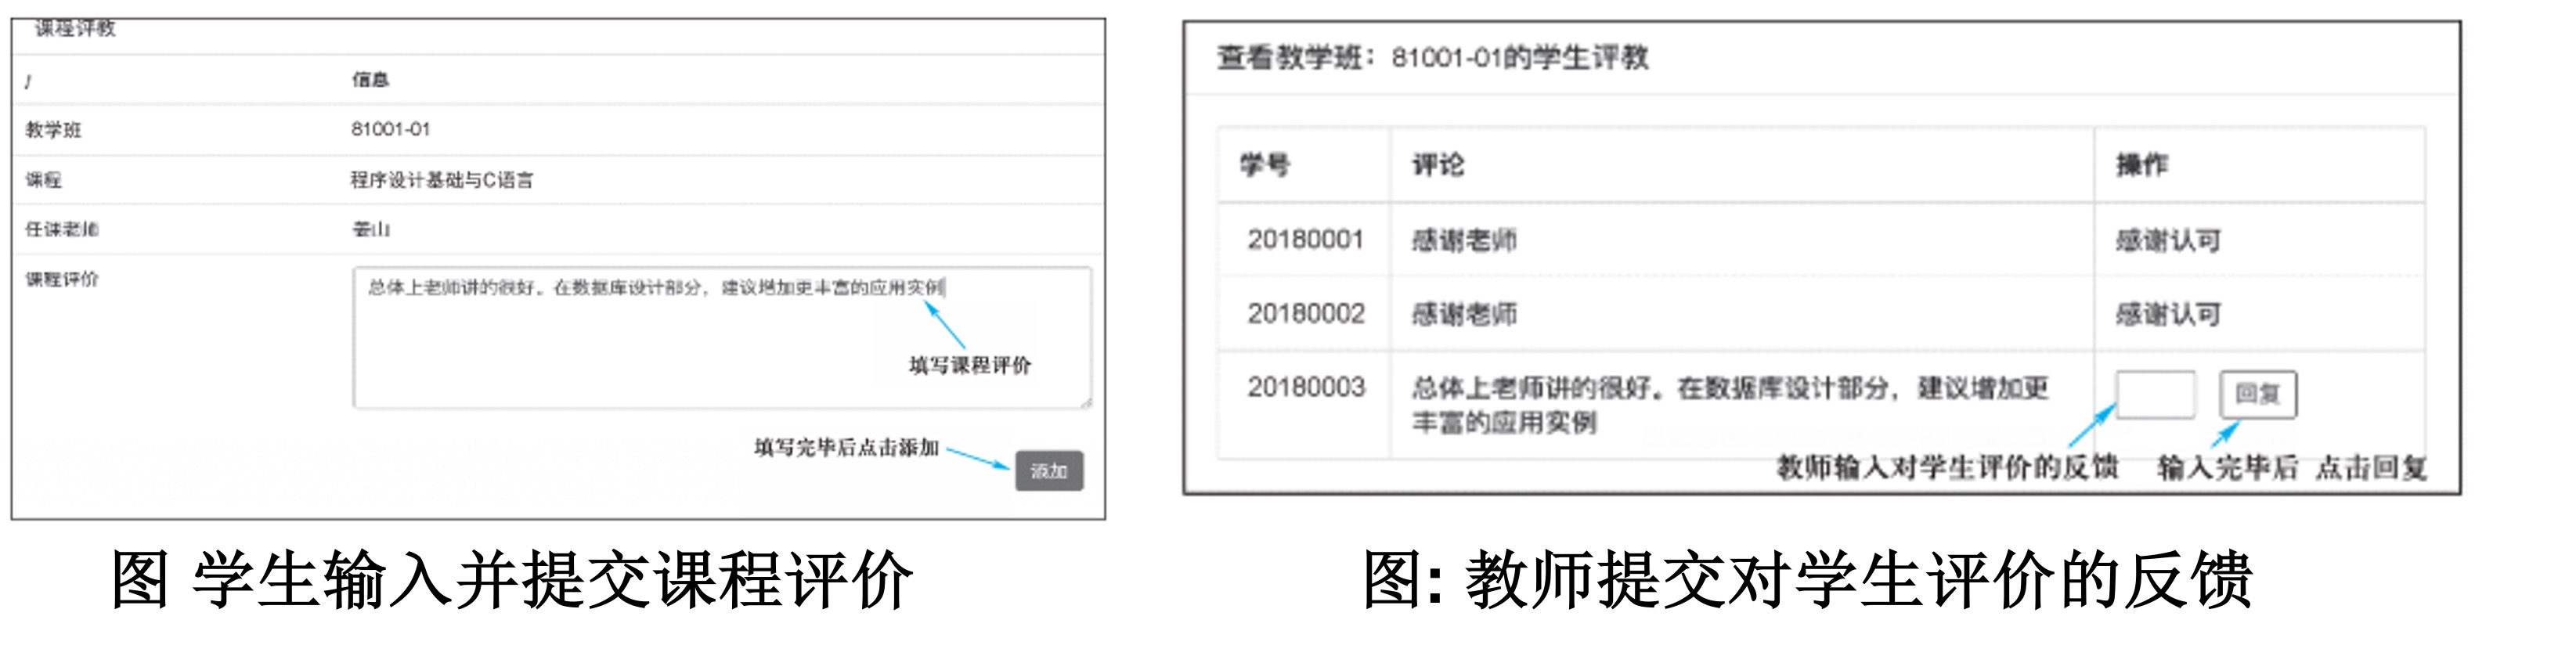
\includegraphics[width=0.8\textwidth]{figure/fig-7.jpg}
\end{figure}

\end{itemize}
\end{itemize}
\end{frame}

\begin{frame}[allowframebreaks]{小结}
\begin{itemize}
    \item SQL语言表达能力的限制
\begin{itemize}
\item 无法表达递归等复杂操作--例如间接先修课的查询
\item 无法对数据进行复杂操作--查询一周内将过生日的同学
\item 无法自主设计业务处理逻辑—计算学生平均学分绩点
\item 无法进行交互式操作--教学评价与反馈
\end{itemize}


\end{itemize}
\end{frame}


\subsection{1.2 扩展SQL的功能}
\begin{frame}[allowframebreaks]{扩展SQL语言的功能}
\begin{itemize}
    \item 1.引入新的SQL子句
    \item 2.引入新的内置函数
    \item 3.引入PL/SQL与存储过程/存储函数
\end{itemize}
\end{frame}

\begin{frame}[allowframebreaks]{引入新的SQL子句}
\begin{itemize}
    \item 以【任务1】为例,SQL标准引入了WITH RECURSIVE子句,可执行递归查询
    \item 类似于WITH RECURSIVE子句的SQL扩展还有很多,例如面向联机分析处理的窗口子句,面向空间数据管理、文档数据管理的SQL语言扩展等
    \item 在介绍WITH RECURSIVE子句之前,先了解WITH子句的用法
\end{itemize}
\end{frame}

\begin{frame}[allowframebreaks,fragile]{WITH子句 格式}
\begin{itemize}
    \item WITH子句的一般格式:
\end{itemize}
    \begin{block}{}
\begin{lstlisting}
WITH RS1[(<目标列>,<目标列>)]AS    /* RS1为临时结果集的命名*/
(SELECT 语句1)[,                  /* RS1对应SELECT 语句的执行结果*/
/*SELECT语句1中的目标列与RS1中的目标列必须保持一致*/
RS2[(<目标列>,<目标列>)]AS        /* RS2为临时结果集的命名*/
(SELECT 语句2),…]                /* RS2对应SELECT 语句的执行结果*/
/*SELECT语句2中的目标列与RS2中的目标列必须保持一致*/
    SQL语句;                      /* 执行与RS1,RS2,…,相关的查询*/
\end{lstlisting}
\end{block} 
\end{frame}

\begin{frame}[allowframebreaks,fragile]{WITH子句 示例}
\begin{itemize}
\item 例: 求81001-01和81001-02两个教学班之间学生选课平均成绩的差异。
\end{itemize}
    \begin{block}{}
\begin{lstlisting}
WITH 
RS1(Grade)
        AS 
        (SELECT AVG(Grade) FROM SC 
        WHERE Teachingclass = '81001-01'),
RS2(Grade)
        AS 
        (SELECT AVG(Grade) FROM SC 
        WHERE Teachingclass = '81001-02')
SELECT RS1.Grade-RS2.Grade FROM RS1,RS2;
\end{lstlisting}
\end{block} 
\end{frame}

\begin{frame}[allowframebreaks,fragile]{WITH RECURSIVE子句 格式}
\begin{itemize}
\item WITH RECURSIVE子句的一般格式:
\end{itemize}

\begin{block}{}
\begin{lstlisting}
WITH RECURSIVE RS AS
    (
        SEED QUERY           /*初始化查询的临时结果集,记为L[1]*/
        UNION [ALL]          /*是否需要保留重复记录,加ALL为保留*/
        RECURSIVE QUERY      
        /*执行递归查询,得到全部临时结果集,即L[2]∪…∪L[i]*/
   ) 
   SQL语句           /*执行与RS相关的查询*/
\end{lstlisting}
\end{block} 

\end{frame}

\begin{frame}[allowframebreaks,fragile]{WITH RECURSIVE子句 示例}
\begin{itemize}
    \item 【任务1】打印“数据库系统概论”课程的所有先修课信息
\end{itemize}
    \begin{figure}
    \centering
    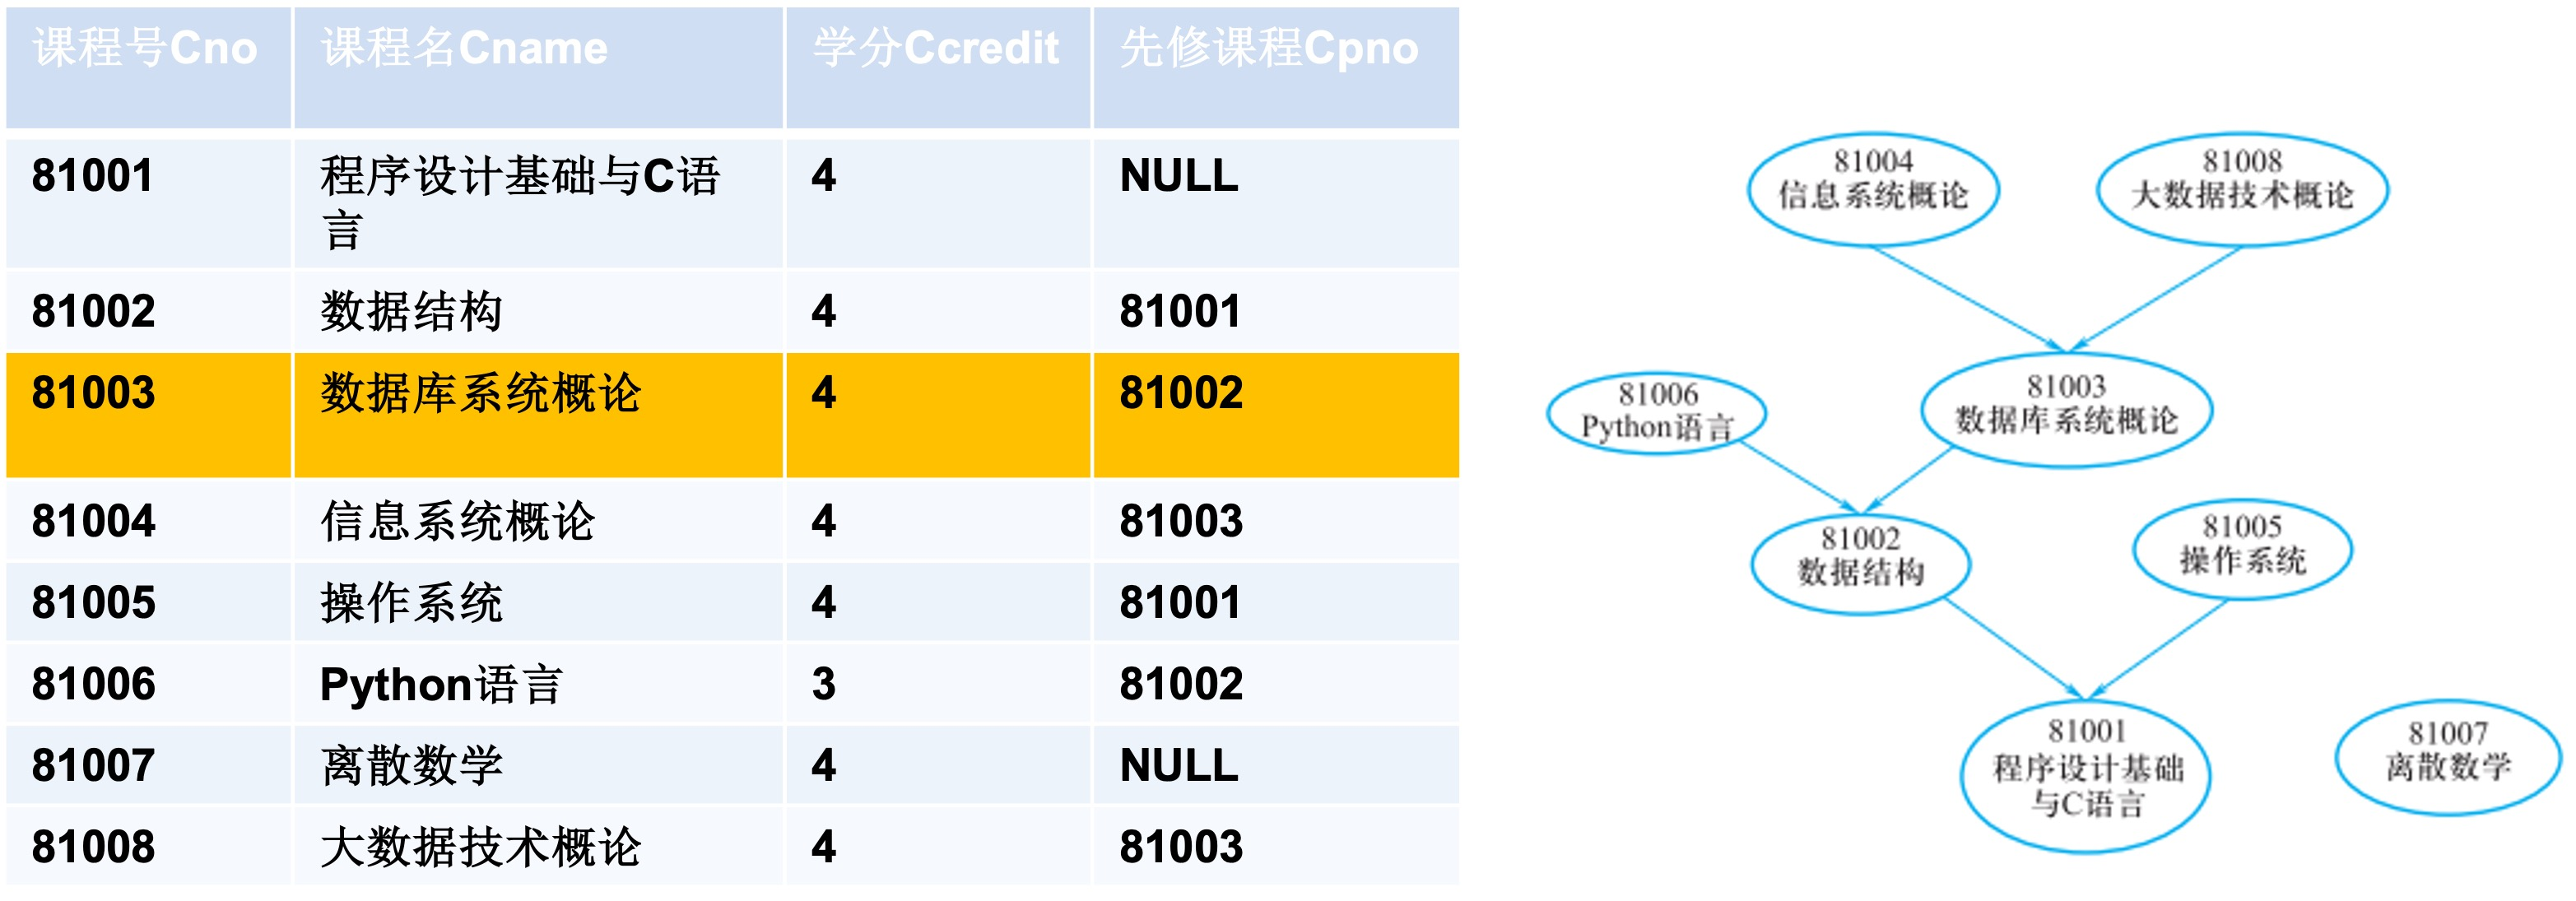
\includegraphics[width=0.9\textwidth]{figure/fig-8.jpg}
\end{figure}

\framebreak
\begin{itemize}
    \item 【任务1】打印“数据库系统概论”课程的所有先修课信息
\end{itemize}

\begin{block}{}
\begin{lstlisting}
WITH RECURSIVE RS AS     
    (SELECT Cpno FROM Course WHERE Cname = '数据库系统概论'
    /*初始化RS,假设结果集为L[1],即“数据库系统概论”的所有直接先修课*/
    UNION  
    SELECT Course.Cpno FROM Course,RS WHERE RS.Cpno = Course.Cno)
    /*递归查询第i层(i>=1)的数据,即第i-1层数据的直接先修课课程号,并更新RS*/
SELECT Cno, Cname FROM Course WHERE Cno IN (SELECT Cpno FROM RS);
/*根据RS中记录的所有先修课程号,通过查找课程表,输出课程号与课程名*/

\end{lstlisting}
\end{block} 
\end{frame}


\begin{frame}{引入新的内置函数}
    \begin{itemize}
        \item SQL常用的内置函数可以分为:
\begin{itemize}
    \item 数学函数(如绝对值函数等)
    \item 聚合函数(如求和、求平均函数等)
    \item 字符串函数(如求字符串长度、求子串函数等)
    \item 日期和时间函数(如返回当前日期函数等)
    \item 格式化函数(如字符串转IP地址函数等)
    \item 控制流函数(如逻辑判断函数等)
    \item 加密函数(如使用密钥对字符串加密函数等)
    \item 系统信息函数(如返回当前数据库名、服务器版本函数等)
\end{itemize}
    \end{itemize}
\end{frame}

\begin{frame}[allowframebreaks,fragile]{日期和时间函数 示例}
    \begin{itemize}
        \item 【任务2】打印一周内将过生日的学生信息
    \end{itemize}

\begin{block}{}
\begin{lstlisting}
SELECT Sno, Sname, Ssex, Sbirthdate, Smajor 
FROM Student 
WHERE to_date(to_char(current_date,'yyyy') || '-' || to_char(Sbirthdate,'mm-dd')) 
BETWEEN CURRENT_DATE AND CURRENT_DATE + INTERVAL '7' DAY;
\end{lstlisting}
\end{block} 
\begin{itemize}
    \item 在WHERE 语句中使用了以下内置函数:
    \begin{enumerate}
        \item 内置函数 \lstinline{current_date} 返回当前的系统日期,例如 2021-6-9
        \item 内置函数 \lstinline{to_char(current_data,'yyyy')}返回当前系统日期的年份,例如 2021; \lstinline{to_char(Sbirthdate,'mm-dd')}返回学生出生日期中具体的月份和日期,例如 6-9
        \item \lstinline{to_date(to_char(current_date,'yyyy')||'-'|| to_char(Sbirthdate,'mm-dd'))}表示把当前年份与出生日期用'-'连在一起。符号\lstinline{'‖'}用于把其左右两边的字符串连在一起
        \item 内置函数 \lstinline{to_date()}的作用是将字符类型按一定格式转化为日期类型。
        \item \lstinline{CURRENT_DATE + INTERVAL '7' DAY}是对当前的日期调整后的日期。参数interval是年(yyyy)、季度(q)、月(m)、日(d)、时(h)等粒度的时间单位。例如,\lstinline{CURRENT_DATE + INTERVAL '7' DAY}获得当前日期之后第七天的日期,即返回2021-6-16
    \end{enumerate}
    \item 通过执行此WHERE语句,判断学生表中每位学生转换后的出生日期是否在[2021-6-9,2021-6-16]区间内,如果是,打印该学生的信息
\end{itemize}
\end{frame}

\begin{frame}{引入PL/SQL与存储过程/存储函数}
    \begin{itemize}
        \item 关系数据库管理系统中引入PL/SQL、存储过程和自定义函数等方法,使得用户可以自定义程序逻辑,开发完成业务逻辑复杂的应用系统。
    \end{itemize}
\end{frame}

\subsection{1.3 通过高级语言实现复杂应用}

\begin{frame}{通过高级语言实现复杂应用}
    \begin{itemize}
        \item 通过动态链接库调用的方式
        \begin{itemize}
            \item 关系数据库管理系统的功能被包装成一个子程序,由应用程序通过动态链接库调用来获得数据管理的功能
        \end{itemize}
        \item 基于嵌入式SQL的方式
        \begin{itemize}
            \item 将SQL嵌入到高级语言中混合编程,SQL语句负责操纵数据库,高级语言语句负责控制逻辑流程
        \end{itemize}
        \item 基于ODBC/JDBC的中间件方式
        \begin{itemize}
            \item 建立了连接不同数据库的一组规范。无论使用什么数据库,都采用同样的一组API来访问数据库
        \end{itemize}
    \end{itemize}
\end{frame}







